\begin{mydef}
	Deux droites sont \hspace*{5cm} si elles n'ont qu'un seul point commun : leur \hspace*{8cm}.
\end{mydef}


\begin{myex}
	\begin{multicols}{2}
		Les droites $(d)$ et $(d')$ sont \hspace*{4cm} en $O$ qui est leur \hspace*{8cm}.
		
		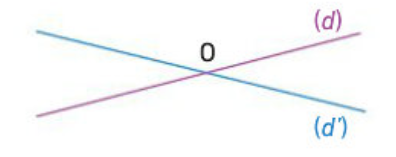
\includegraphics[scale=0.5]{img/sec}
	\end{multicols}
	
\end{myex}

\begin{mydef}
	Deux droites sont \hspace*{5cm} si elles se coupent en formant \hspace*{8cm}. Si deux droites $(d_1)$ et $(d_2)$ sont deux droites perpendiculaires, on note $(d_1) \bot (d_2)$.
\end{mydef}

\begin{myex}
	\begin{multicols}{2}
		Les droites $(d)$ et $(d')$ sont \hspace*{6cm} en $H$. $H$ est le \hspace*{8cm} à $(d')$.
		
		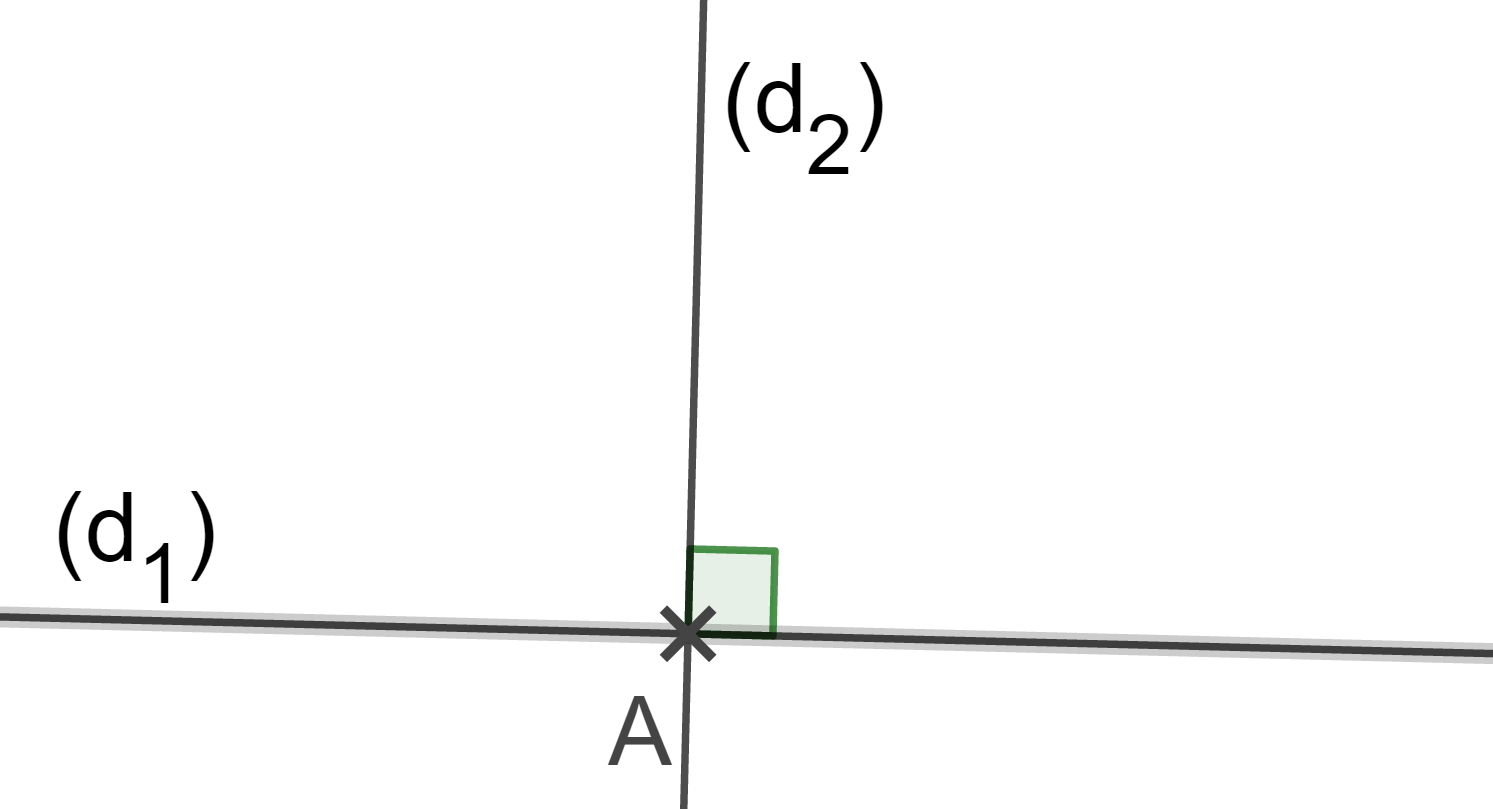
\includegraphics[scale=0.6]{img/perp}
	\end{multicols}
	
\end{myex}

\begin{mydef}
	Deux droites qui ne sont pas sécantes sont \hspace*{6cm}. Si deux droites $(d_3)$ et $(d_4)$ sont parallèles, on note $(d_1) // (d_2)$.
\end{mydef}

\begin{myex}
	\begin{multicols}{2}
		Les droites $(d)$ et $(d')$ sont \hspace*{5cm}. Même en les prolongeant à l'infini elles ne se rencontreront jamais.
		
		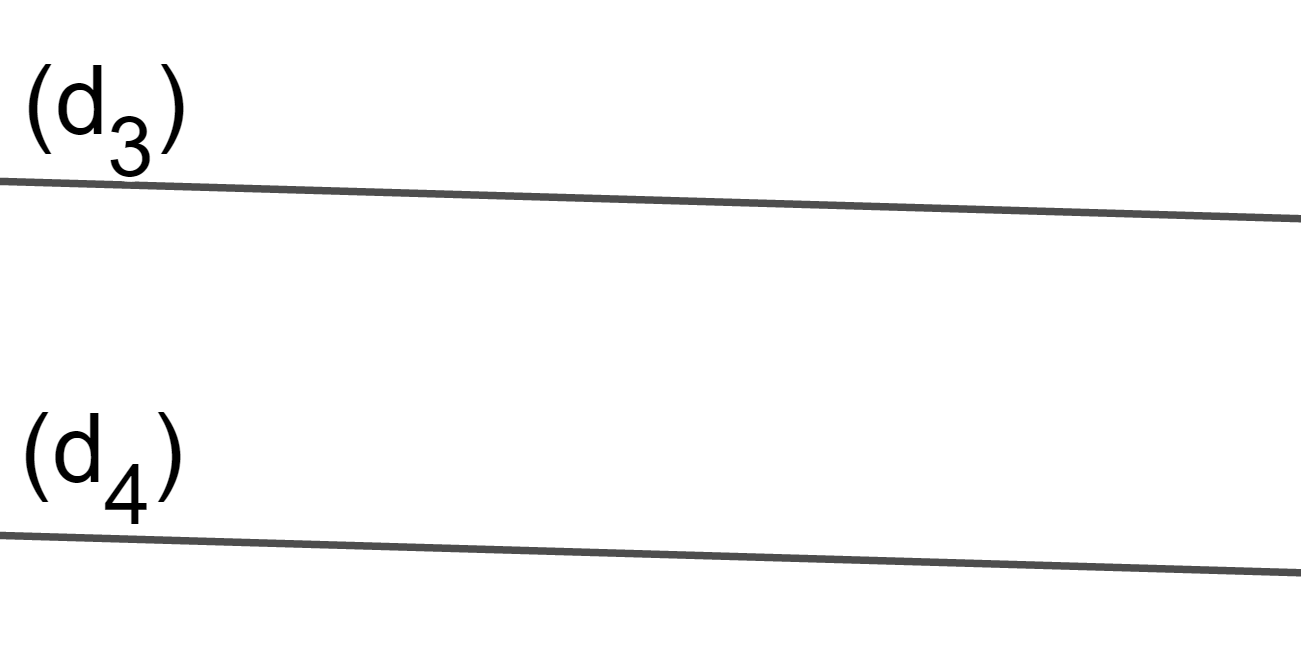
\includegraphics[scale=0.6]{img/para1}
	\end{multicols}
	
\end{myex}

\begin{myprop}
	\kw{Si} deux droites sont \hspace*{6cm} à une \hspace*{8cm}, \kw{alors} ces deux droites sont \hspace*{6cm}.
\end{myprop}


\begin{myex}
	\begin{multicols}{2}
		\kw{On sait que} $(d_1)$ et $(d_2)$ sont toutes deux perpendiculaires à $(D)$.\\
		\kw{Donc} $(d_1)$ et $(d_2)$ sont parallèles.
		
		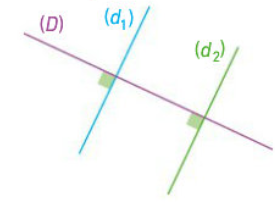
\includegraphics[scale=0.6]{img/para2}
	\end{multicols}
	
\end{myex}